\documentclass{LxUm}
 
% ----------------------------------------------------------------
% Beginn
% ----------------------------------------------------------------
\begin{document}
 
% ----------------------------------------------------------------
% Zeilenabstand \onehalfspacing\doublespacing\singlespacing
% ----------------------------------------------------------------
\singlespacing

% ----------------------------------------------------------------
% Stil fuer Fusszeile
% ----------------------------------------------------------------
\pagestyle{fancy}

% ----------------------------------------------------------------
% Schriftart
% ----------------------------------------------------------------
\sffamily

% ----------------------------------------------------------------
% Titelseite
% ----------------------------------------------------------------
\newpage%
\thispagestyle{empty}%
\part*{Regelungstechnik A \\(Grundlagen und Frequenzbereichsmethoden)}%
\newpage%Ayke Darius geschrieben:


% ----------------------------------------------------------------
% Hauptteil
% ----------------------------------------------------------------
\chapter{Gegenstand der Regelungstechnik} Die Regelungstechnik (RT) besch�ftigt sich mit der selbstt�tigen gezielten Beeinflussung des
Verhaltens von dynamischen Systemen.

\begin{center}
	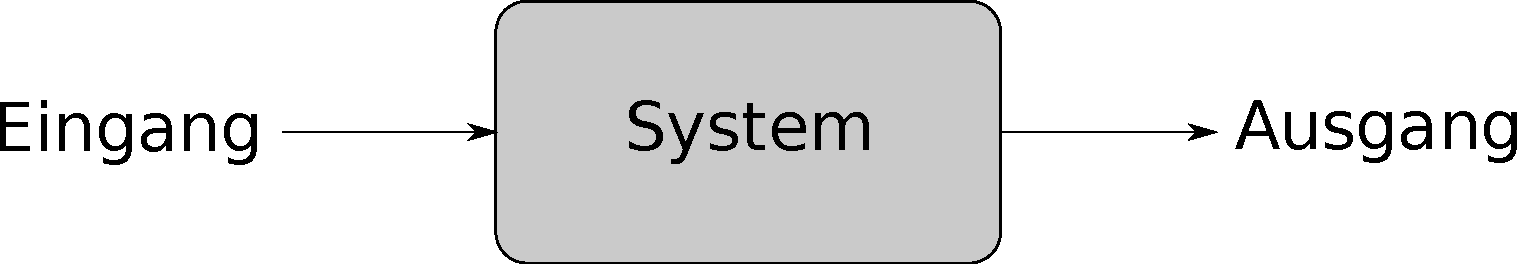
\includegraphics[width=300px]{graphics/system1.pdf}
\end{center}

Die Eing�nge werden in der RT aufgeteilt in von au�en vorgebbare \underline{Eingangsgr��en} und in durch die Umgebung festgelegte, st�rend wirkende \underline{St�rgr��en}. Von den Ausg�ngen werden nur diejenigen betrachtet, deren Verhalten unmittelbar interessiert. \underline{Ausgangsgr��en}.

\begin{center}
	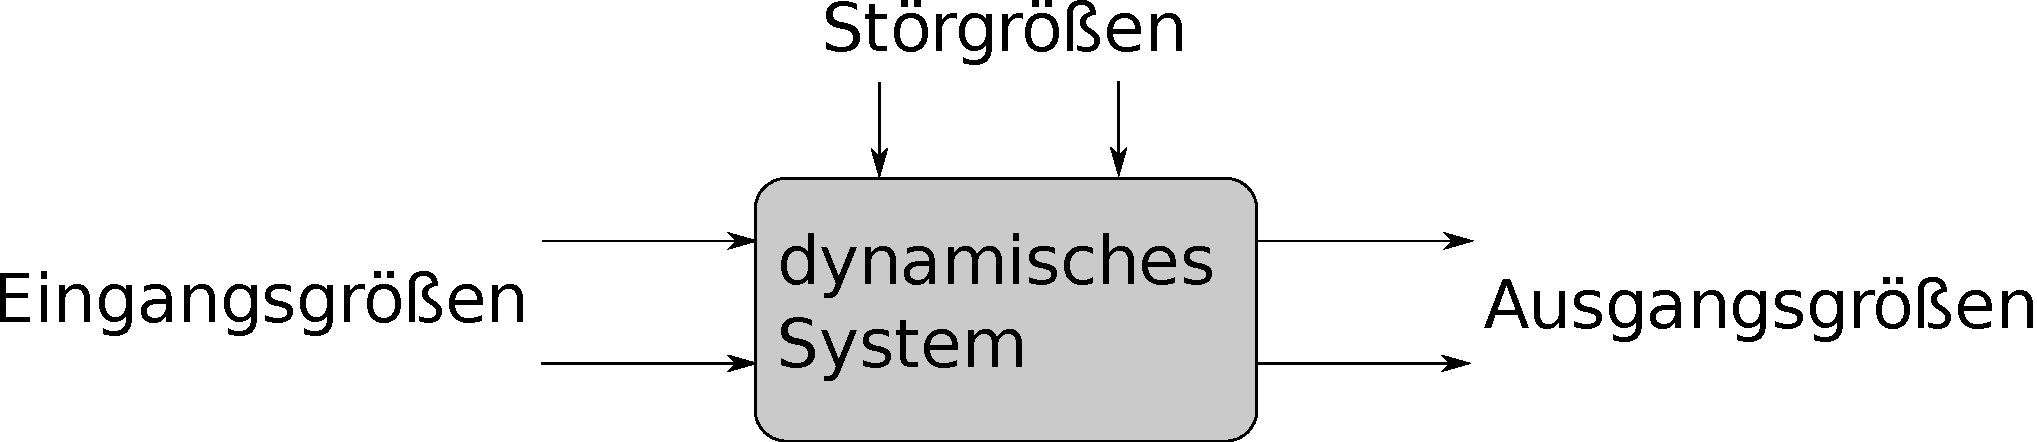
\includegraphics[width=300px]{graphics/dynsystem1.pdf}
\end{center}

\underline{Gezielte Beeinflussung} hei�t: Durch Vorgabe der Eingangsgr��enverl�ufe soll erreicht werden, dass die Ausgangsgr��en trotz St�reinwirkung ein gew�nschtes \underline{Sollverhalten} aufweisen.

\subsubsection*{Beispiel 1 (Raumtemperatur)}
\begin{center}
	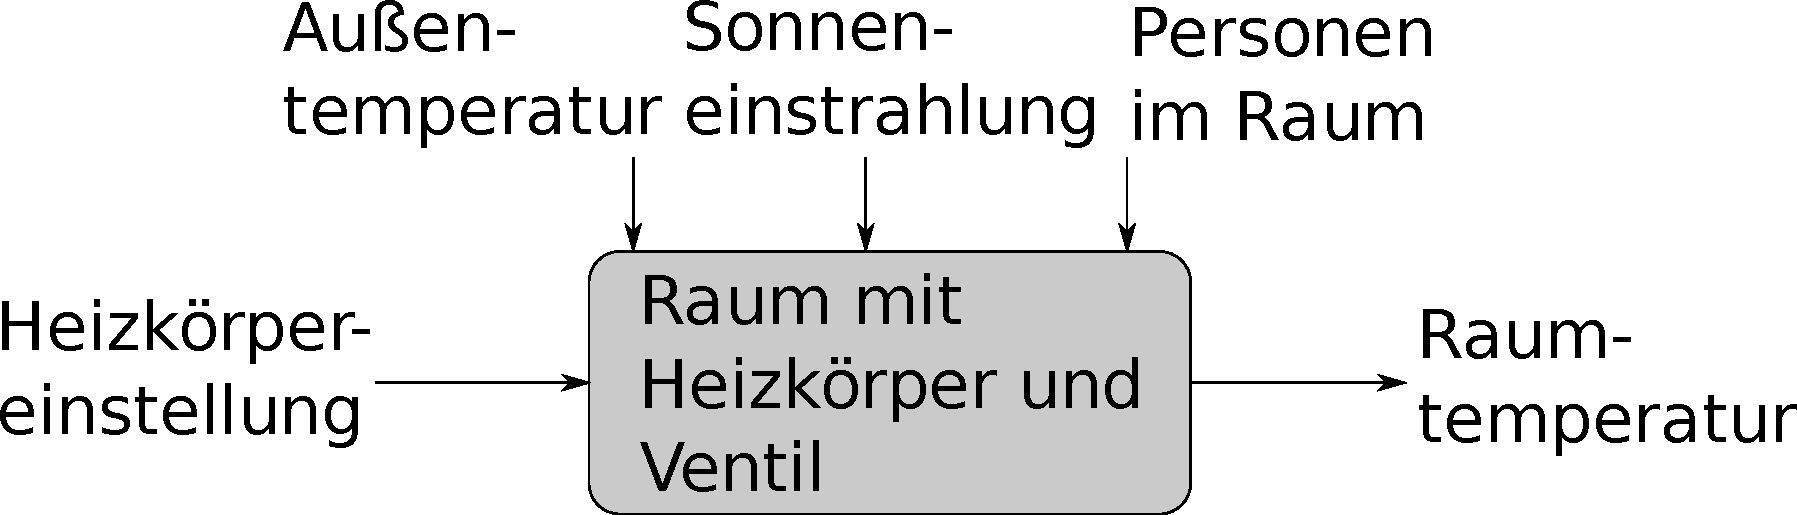
\includegraphics[width=300px]{graphics/raumtemperatur.pdf}
\end{center}

\subsubsection*{Beispiel 2 (Personenaufzug)}
\begin{center}
	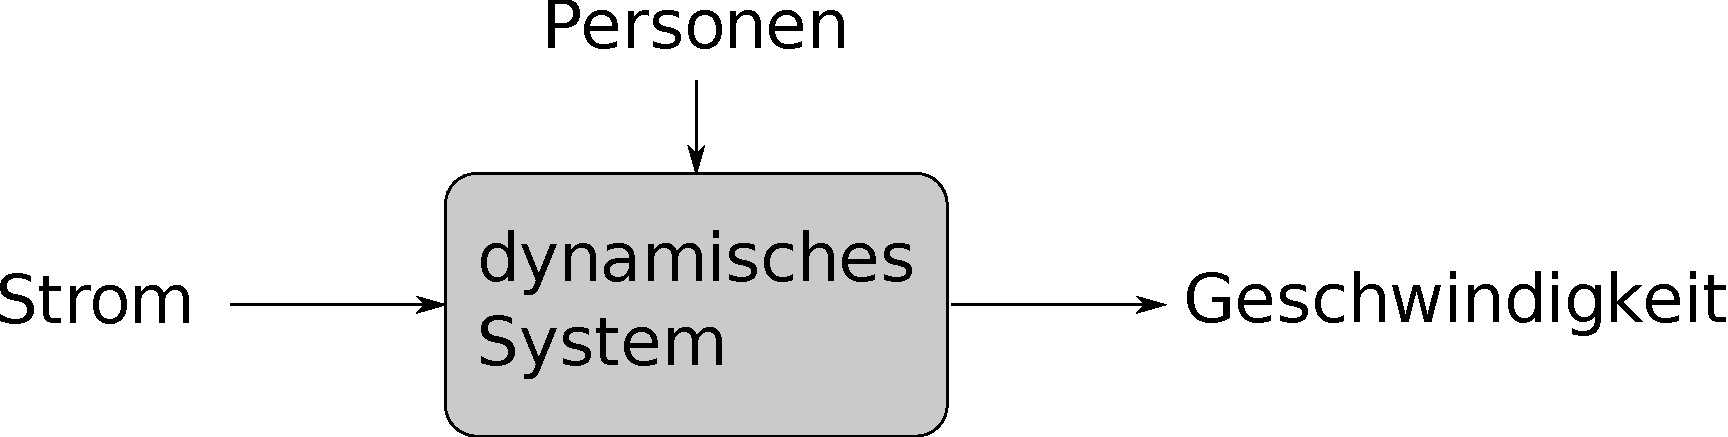
\includegraphics[width=300px]{graphics/personenaufzug.pdf}
\end{center}

\subsubsection*{Beispiel 3 (Auto fahren)}
\begin{center}
	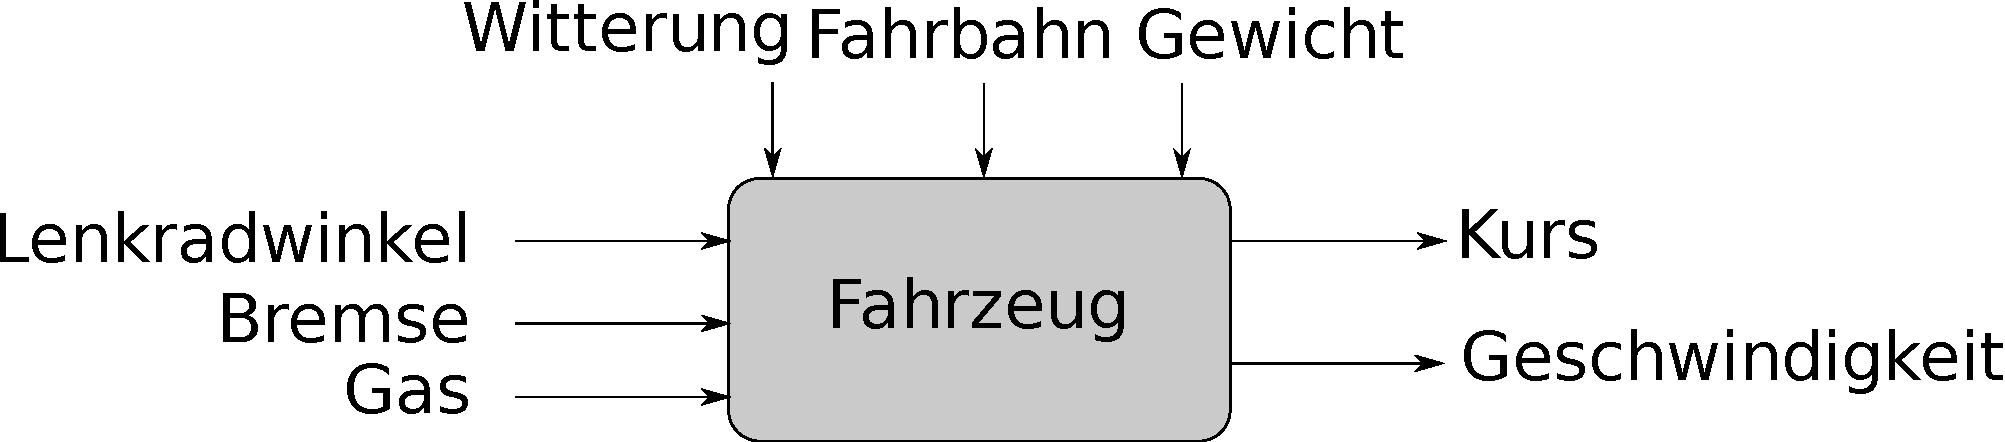
\includegraphics[width=300px]{graphics/autofahren.pdf}
\end{center}

\section*{Allgemeine Aufgabenstellung der RT}
Entwurf und Bereitstellung einer Einrichtung, die - hinzugef�gt zur Strecke - die Eingangsgr��en automatisch im gew�nschten Sinne generiert. \underline{Selbstt�tige gezielte Beeinflussung}.

\section*{Generelle Vorgehensweise zur L�sung}
\begin{enumerate}
	\item{mathematische Modellbildung der Strecke zur Abstraktion von deren physikalischen Auspr�gung und Erm�glichung der Anwendung universell einsetzbarer, systemtheoretisch fundierter Vorgehensweisen in Schritt 2. und 3.}
	\item{Analyse des Streckenverhaltens}
	\item{Entwurf der Steuer- und Regeleinrichtung}
	\item{Realisierung der Steuer- und Regeleinrichtung}
	\item{Inbetriebnahme und Erprobung des Gesamtsystems}
\end{enumerate}

\chapter{Modellbildung der Strecke} \begin{thms}
	Modellbildung der Strecke durch mathematische Beschreibungen der Wirkungszusammenh�nge zwischen den Systemgr��en, die f�r die Aufgabenstellung relevant sind.
\end{thms}

Ein Modell ist eine aufgabenspezifische Vereinfachung der Realit�t. In der RT bew�hrte Modellierungsform:

\section{Darstellung der Strecke als Strukturbild (Blockschaltbild)}
\subsection{Beispiel: Permant erregter Gleichstrommotor}
\begin{itemize}
	\item Ger�teschema: (siehe Beiblatt 4)
	\item Systemdarstellung:
\end{itemize}

\begin{center}
	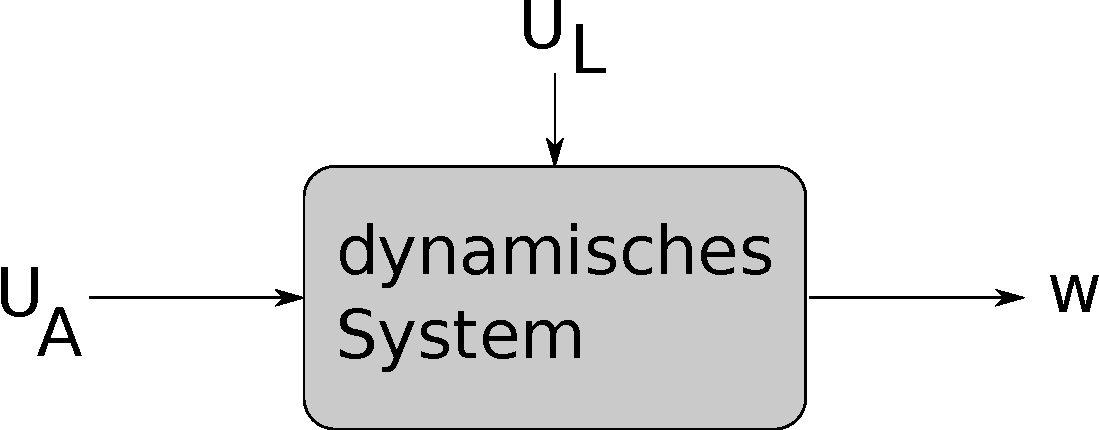
\includegraphics[width=200px]{graphics/gleichstrommotor.pdf}
\end{center}

\subsubsection{Ermittlung der beschreibenden Gleichungen:}

  \[u_l(t) = L \frac{di_A(t)} {dt} \longrightarrow \frac{d i_A(t)}{dt} = \frac{1}{L_A} u_l(t) \]
\begin{equation}
   \xrightarrow {\text{Integration von 0 bis t}} i_A(t) = i_A(0) + \frac{1}{L_A} \int_0^t u_l(\tau), d \tau 
\end{equation}
 \[u_A(t) = u_R + u_L + u_{ind} \]
\begin{equation}
\longrightarrow u_L(t) = u_A(t) - u_R(t) - u_{ind}(t)
\end{equation}

\begin{equation}
 u_R(t) = R_A i_A(t)
\end{equation}

\begin{equation}
 u_{ind}(t) = c \phi_F \omega(t)
\end{equation}

\subsubsection*{Rotierender Anker + Welle:}
\[J\dot{\omega} = M_\Sigma
\longrightarrow \dot{\omega} = \frac{1}{J} M_\Sigma(t) \]
\begin{equation}
 \xrightarrow {\text{Integration von 0 bis t}}  \omega(t) = \omega(0) + \frac{1}{J} \int_0^t M_z(\tau), d \tau
\end{equation}

		\begin{center}
			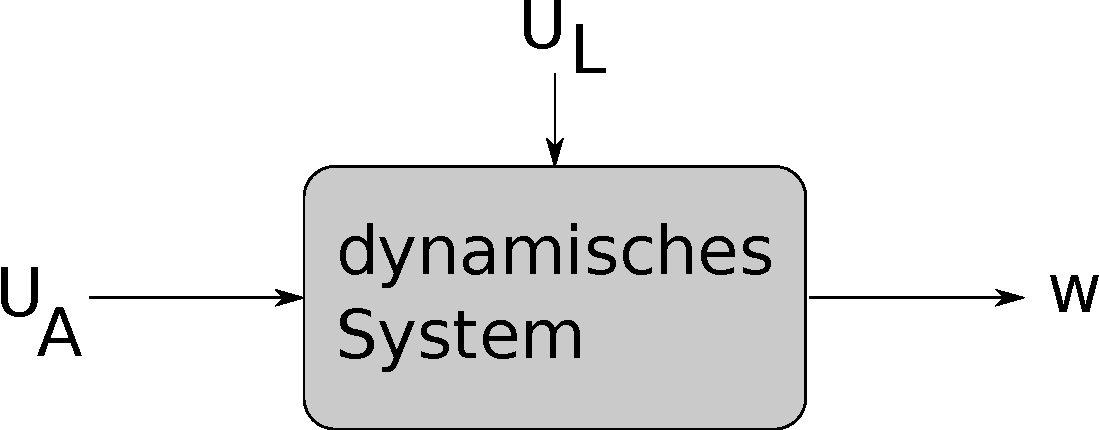
\includegraphics[width=200px]{graphics/gleichstrommotor.pdf}
		\end{center}
\begin{itemize}
		\item Ermittlung der beschreibenden Gleichungen:
		\subitem Ankerstromkreis
		\begin{align}
		u_L=L\frac{di_A}{dt} \rightarrow \frac{di_A(t)}{dt}=\frac{1}{L}u_L(t) \stackrel{\int_0^t}{\rightarrow}i_A(t)=i_A(0)+\frac{1}{L_A}\int_0^t u_L(\tau)d\tau \\
		u_A=u_R+u_L+u_{ind} \rightarrow u_L(t)=u_A(t)-u_R(t)-u_{ind}(t) \\
		u_R(t)=R_Ai_A(t) \\
		U_{ind}=c\phi\omega(t)
		\end{align}
		\subitem Rotierender Anker und Welle
		\begin{align}
		J\dot{\omega}=M_{\sum} \rightarrow \dot{\omega}(t)=\frac{1}{J}M_{\sum}(t)\stackrel{\int_0^t}{\rightarrow}\omega(t)=\omega(0)+\frac{1}{J}\int_0^t M_{\sum}(\tau)d\tau \\
		M_{\sum}(t)=M_A(t)-M_L(t) \\
		M_A(t) = c \phi_F L_A(t)
		\end{align}
	\item �bersetzung der Gleichungen ins Strukturbild {TODO:BILD}
	\begin{thms}
		Strukturbild = Graphische Darstellung der Systemregeln (durch Bl�cke und Wirkungslinien). Dadurch anschaulich und \underline{Wirkungsrichtungen} sofort ersichtlich.
	\end{thms}
\end{itemize}

\subsection{Die Bausteine des Strukturfeldes}
\begin{itemize}
	\item \underline{gerichtete Linien} geben die \underline{Systemgr��en im Zeitbereich} und ihre Wirkrichtungen wieder
	\item \underline{Bl�cke, Rechtecke und Kreise} beschreiben die Funktionsbeziehung zwischen den Systemgr��en und ordnen jedem Zeitverlauf der Eingangsgr��en
eindeutig einem Zeitverlauf der Ausgangsgr��e zu. \\
	$ \rightarrow {\text{Jeder Block wirkt als \underline{�bertragungsglied} (�G)}} $

\end{itemize}

\subsubsection{Darstellungsm�glichkeiten}
\begin{itemize}
 \item mittels Zuordnungsvorschrift bzw. Systemoperator $\boldsymbol{\mathcal{S}}$ (vgl. obiges Beispiel)
	\begin{equation*}
		y(t) = \mathcal{S}\left \{ u(t)  \right \}
	\end{equation*}
	\TODO{Blockdiagramm}

 \item bei LZI-�G weiterhin
	\subitem mittels �bertragunsfunktion �G 
	\begin{equation*}
		y(t) \multimapdotbothA Y(s) = G(s)U(s)
	\end{equation*}
	\TODO{Blockdiagramm}

	\subitem mittels Sprungantwort $y_\sigma(t)$ (= $ y(t) $ f�r $ u(t) $ = Einheitsprung $ \sigma(t) $ )
	\begin{align*}
		y(t) = g(t)*u(t)  = \dot{y}_\sigma(t) * u(t) \\
		\mbox{(da $ g(t) = \dot{y}_\sigma(t) $ gilt.)}
	\end{align*}
	\TODO{Blockdiagramm}

 \item Zusammenstellung elementarer �G \\
	(nicht in noch einfachere Bestandteile zerlegbar):\\
	$\rightarrow$ siehe \bb{5}
\end{itemize}

\begin{hinweis}[Totzeitglied]
	\begin{itemize}
		\item typisch f�r Transportprozesse
		\item �F rational approximierbar z.B. gem��
		\[ e^{-T_t s} \approx \frac{1- 0,5 T_t s}{1 + 0,5 T_t s} \]
	\end{itemize}
\end{hinweis}

H�ufig auftretende Kombinationen elementarer �G werden zu \underline{zusammengesetzten} �G zusammengefasst. $\rightarrow$ siehe \bb{6}

\subsubsection{Aufbau des $PT_1$ - Gliedes aus elementaren �G}
\begin{align}
    T\dot{y} + y = Ku \\
    \rightarrow \dot{y} = \frac{1}{T} (K u - y) = \frac{K}{T} (u - \frac{1}{K} y) \\
    y(t) = y(0) + \frac{K}{T} \int_0^t v(\tau) d\tau   \text{ mit } v(t) = u(t) - \frac{1}{K} y(t)
\end{align}
\TODO{Blockschaltbild}

\subsubsection{Normierte $PT_2$-Sprungantworten f�r $D\le 1$}
$\rightarrow$ siehe \bb{7}

\subsection{Weiteres Beispiel: Magnetlager als Fahrzeug Tragsystem}
\begin{itemize}
 \item Ger�teschema siehe $\bb{8}$ \\
	\TODO Blockdiagramm
 \item Beschreibende Gleichungen und Strukturbild siehe $\bb{9}$ \\
\end{itemize}

\section{Modellvereinfachung durch Betriebspunkt-Linearisierung}
\subsection{Betriebspunkt bzw. Arbeitspunkt eines Systems}
\begin{itemize}
 \item \underline{Betriebspunkt (BP)} = System-Ruhezustand, in dem die Ausgagsgr��e y den station�ren Sollwert $y_{s\infty}$ annimmt.
 \item \underline{Ruhezustand} (Ruhelage, Gleichgewichtslage, station�rer Zustand) = Systemzustand, in dem \underline{alle} Systemgr��en konstant
und damit ihre Zeitableitung gleich null sind. Zu seiner Bestimmung entweder die Systemgleichungen heranziehen und darin dei Ableitungen null 
setzen oder im Strukturbild in der �bertragunsfunktion $s=0$ setzen, au�er beim $\boldsymbol{I-Glied}$:\\
 \item Dort muss die Eingangsgr��e Null sein. F�r die BP-Bestimmung dann noch $y \stackrel{!}{=} y_{s\infty}$ setzen.
\end{itemize}
\subsubsection{Beispiel Magnetlager}
\begin{itemize}
 \item F�r $F_{zb} = 0$ soll $x_B = x_{s\infty} = \frac{d}{2}$ gelten. \\
 \item Einzustellendes $i$? \\
	\[
	\left.\begin{matrix}
	    v_B = 0 \\
	    F_{\Sigma B} =  
	\end{matrix}\right\}
\xrightarrow[]{F_{zB} = 0} F_{mB} = mg \]
\[F_{mB} = K_m \frac{i_B^2}{(d-x_B)^2} \xrightarrow[x_B = \frac{d}{2}] {F_{mB} = mg} i=\sqrt{\frac{mg}{K_m}} \cdot \frac{d}{2} \]

\end{itemize}

\subsection{Durchf�hrung der Linearisierung}
\begin{enumerate}
 \item \underline{�bergang von den Absolutgr��en $u(t)$, $y(t)$ zu den BP-Abweichungen}
	\[ \Delta u(t) = u(t) - u_B \\
	 \Delta y(t) = y(t) - y_B
	\]
Ein lineares �G $y(t) = \mathcal{S} \left \{ u(t) \right \} $ geht dabei �ber in 
\begin{align}
	\Delta y(t) &= y(t) - y_B \\
	&= \mathcal{S} \left \{ u(t)  \right \} - \mathcal{S} \left \{ u_B  \right \} \\
	&= \mathcal{S} \left \{ u_B  \right \} +  \mathcal{S} \left \{ \Delta u(t) \right \} - \mathcal{S} \left \{ \Delta u_B \right \}
\end{align}
\[ \rightarrow \Delta y(t) =  \mathcal{S} \left \{ \Delta u(t) \right \}\]
d.h. \underline{lineare �G bleiben unver�ndert} \\
F�r ein nicht lineares �G folgt: \\
\begin{align}
	\Delta y(t) & = \mathcal{S} \left \{ u_B(t) + \Delta u(t) \right \} - \mathcal{S} \left \{ u_B \right \} \\
	& = \mathcal{\tilde S} \left \{ \Delta u(t) \right \} \not= \mathcal{\tilde S} \left \{ \Delta u(t) \right \}
\end{align}

d.h. \underline{Nichtlineare �G �ndern dabei ihre Funktionalbezieung, bleiben aber i.A. nichtlinear} \\

\subsubsection{Beispiel: KL-Glied $y=F(u)$}

\TODO Graph

\item \underline{Schritt:}\\
Annahme kleiner Abweichungen und lineare Approximation der nichtlinearen Beziehungen durch Taylor-Reihenentwicklung mit Abbruch nach dem linearen Term \\
z.B. KL-Glied
\begin{align}
  y(t)  = F(u(t)) \xrightarrow[]{u = u_B + \Delta u} \\
  y(t)  = F(u_B + \Delta u(t)) \\
  y(t)  = \underbrace{F(u_B)}_{y_B} + F'(u_B) \cdot \Delta u(t) + R(\Delta u(t)^2) \\
\end{align}
Linearisierung durch Weglassen des Restglieds

$\rightarrow$ \underline{nichtlineare �G} gehen in P-Glieder mit der Verst�rkung $F'(u_B)$ �ber.
\end{enumerate}

\subsubsection{\underline{Beispiel Magnetlager}}
\begin{itemize}
 \item Linearisierung der Magnetkraft-Beziehung
	\[ F_M = F_M(i,x) \xrightarrow[i=i_B+\Delta i]{x = x_B + \Delta x} F_M = F_M(i_B, x_B) +  
	\left. \frac{\delta F_M}{\delta i} \right|_B \Delta i + 
	\left. \frac{\delta F_M}{\delta x} \right|_B
	 - \Delta x \]
	\[\rightarrow \Delta F_M = F_M - F_MB = K_i \Delta i + K_x \Delta x mit \]
	\[K_i = \left. \frac{\delta F_M}{\delta i} \right|_B = 2K_m \frac{i_B}{(d-x_B)^2} = ... = 4\frac{\sqrt{mgK_m}}{d} \]
	\[K_x = \left. \frac{\delta F_M}{\delta x} \right|_B = 2K_m \frac{i_B^2}{(d-x_B)^3} = ... = 4\frac{mg}{d} \]

\item Betrachtung der Kr�ftesumme:
	\[ F_\Sigma = F_M -mg - F_z\]
	\[ \xrightarrow{} F_{zB} + \Delta F_\Sigma = F_{MB} + \Delta F_M - mg - F_{zB} - \Delta F_z \]
	\[ \xrightarrow{} \Delta F_\Sigma = \Delta F_M -  \Delta F_z \]
	
\item Strukturfeld des linearisierten Systems

\TODO {Strukturfeld des linearisierten Systems }

\end{itemize}

\section{Modellvereinfachung der Strukturbildumformung}
\begin{itemize}
 \item Beispiel Magnetlager; siehe \bb{10}
\begin{align}
	\Delta X(s) &= \frac{\frac{1}{m}}{s^2} (R(s) + K_x \Delta X(s)) \rightarrow \Delta X(s) = 
	\frac{\frac{\frac{1}{m}}{s^2}}{1-\frac{\frac{1}{m}}{s^2}K_x} R(s) - 1 \frac{1}{K_x} \\
	&= \frac{-\frac{1}{K_x}}{1-(\frac{m}{K_x})s^2}R(s)
\end{align}
	\item \underline{2 Umformungsgrundoperationen:}\\
	Vertauschen der Reihenfolge von �G und \underline{Zusammenfassen}
	mehrere �G. Dabei geltende elementare Regeln: siehe \bb{11}
	\item Alternative zur Umformung im Strukturfeld:
	beschreibende Gleichungen aus Strukturbild ablesen, ineinander einsetzen und nach $y$ als Funktion
	von $u$ und $z$ aufl�sen, dann R�ck�bersetzung in ein Strukturbild.
	Beispiele dazu: siehe \bb{12}
\item Meist Kombination beider Vorgehensweisen!
\end{itemize}


\section{Allgemeines Strukturbild linearer Eingangr��enstrecken}
\begin{itemize}
 \item entspricht dem gemeinsamen Aufbau beider Beispielsysteme, d.h
	\TODO{Strukturbild}
\end{itemize}









\chapter{Analyse des Streckenverhaltens} am Beispiel des Stellverhaltens mit der �F $G(s) = G_1 G_2 $

\section{Betrachtung der Strecken �F}
\subsection{Polynomform der �F}
\TODO{Formeln}

Da im allgemeinen \TODO{Formeln}, ist $\delta$ ein Ma� f�r die verz�gernde Wirkung eines Systems (siehe BB 13)

\subsection{Pol- Nullstellenform der �F}
Sind $n_1,...,n_m$ bzw. $p_i,...,p_n$ die (reellen oder konjugiert komplexen) Wurzeln von $Z(s)=0$ bzw. $N(s)=0$

% ----------------------------------------------------------------
% Ende
% ----------------------------------------------------------------
\end{document}
